\thispagestyle{fancy}
\vspace*{40 pt}
\section{\large{\MakeUppercase{Telas IHM alimentação}}}
Devido ao tamanho reduzido desta tela, não foi possível inserir todas as funcionalidades disponíveis na 
\ifmachineType
 IHM do Slotter e da entrada da Contagem.
\else
 IHM da Corte e Vinco e do Empilhador.
\fi
 Porém um grande trabalho de UX foi realizado para que o operador pudesse realizar todas as tarefas necessárias para o ajuste da unidade mantendo
 o estilo e navegação da IHM das telas grandes. Na IHM da alimentação, o operador pode realizar apenas alguns ajustes da unidade e máquina e existem
 alguns ajustes que são realizados apenas por esta tela por questões de facilidade de acesso e de se tratar de ajustes que requerem visualização pois
 não possuem encoders para ajuste automático.
 
\subsection{Tela principal}\label{ihmAlimentacaoTelaPrincipal}

Na tela principal possui os botões de acesso as telas de ajustes e comandos da unidade por meio do menu esquerdo superior, também é possível acessar
os alarmes por meio do botão esquerdo inferior, estes menus permanecem iguais em todas as telas. Além disso, é possível visualizar algumas informações 
sobre o pedido atual, como o nome do pedido, a quantidade de caixas a serem produzidas, a quantidade de caixas produzidas, a quantidade de caixas
do pedido anterior e a quantidade de caixas produzidas por minuto (velocidade da máquina). Também é possível ajustar a velocidade da máquina clicando
sobre o campo de velocidade e utilizando o teclado numérico para inserir o valor desejado.

\vspace*{\fill}
\begin{figure}[h]
  \centering
  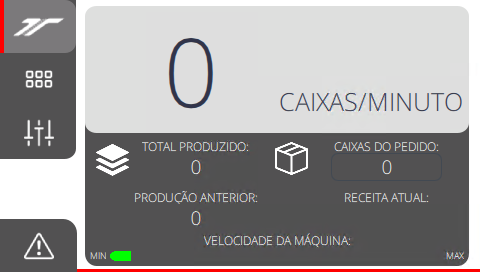
\includegraphics{src/imagesFlexo/11-IHMALM/e-1.png}
\end{figure}
\vspace*{\fill}

\newpage
\thispagestyle{fancy}
\vspace*{40 pt}
\subsection{Tela de comandos página 1}\label{ihmAlimentacaoTelaComandosPagina1}

Para acessar esta tela basta clicar no botão do meio do menu esquerdo superior (destacado na imagem abaixo).
 Na tela de comandos é possível visualizar os comandos disponíveis para a unidade, entre tais:

\newlist {commandsInFeeder}{itemize}{1}
\setlist [commandsInFeeder]{label={}, nosep, before=\vspace{10pt}, after=\vspace{10pt}}

 \begin{commandsInFeeder}
    \item[\ding{\dingNumber}] \textbf{Habilita alimentação de chapas}: habilita a alimentação de chapas para o aparelho;
    \item[\ding{\dingNumber}] \textbf{Habilita skip feed}: lança uma caixa e "pula" a próxima;
    \item[\ding{\dingNumber}] \textbf{Habilita barra eletrostática}: habilita a barra eletrostática removendo partiículas de poeira da chapa;
    \item[\ding{\dingNumber}] \textbf{Habilita esquadrejador}: habilita o esquadrejamento da pilha;
    \item[\ding{\dingNumber}] \textbf{Liga vácuo alimentação}: liga o vácuo da alimentação, permite o lançamento de caixas;
    \item[\ding{\dingNumber}] \textbf{Liga vácuo transporte}: liga o vácuo do transporte, permite o transporte de caixas.
 \end{commandsInFeeder}


\vspace*{\fill}
\begin{figure}[h]
  \centering
  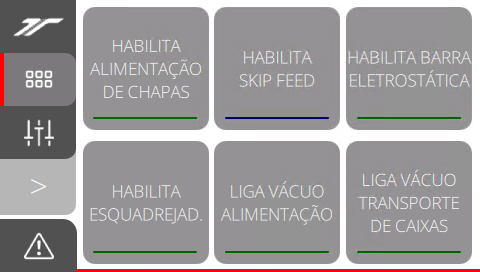
\includegraphics{src/imagesFlexo/11-IHMALM/e-2.png}
\end{figure}
\vspace*{\fill}

\newpage
\thispagestyle{fancy}
\vspace*{40 pt}
\subsection{Tela de comandos página 2}\label{ihmAlimentacaoTelaComandosPagina2}

Esta tela é acessada pelo botão "\textgreater" no menu esquerdo superior na tela de comando. A lógica dos outros menus continua sendo a mesma da sua tela "pai" e para voltar a tela anterior basta clicar no botão esquerdo "\textless{}".

Nesta tela é possível visualizar os comandos disponíveis para a unidade e para ajustes do ecrã, entre tais:


\newlist {commandsInFeeder2}{itemize}{1}
\setlist [commandsInFeeder2]{label={}, nosep, before=\vspace{10pt}, after=\vspace{10pt}}


 \begin{commandsInFeeder2}
    \item[\ding{\dingNumber}] \textbf{Ponto zero LCX (lançador de caixas)}: ajusta o ponto zero do LCX;
    \item[\ding{\dingNumber}] \textbf{Aumentar o brilho da tela}: aumenta o brilho da tela;
    \item[\ding{\dingNumber}] \textbf{Diminuir o brilho da tela}: diminui o brilho da tela;
    \item[\ding{\dingNumber}] \textbf{Habilita o modo limpeza}: habilita o modo limpeza, a tela deixa de ser sensível ao toque por 30 segundos. Permitindo a limpeza da tela;
    \item[\ding{\dingNumber}] \textbf{Sair do runtime}: para o runtime e retorna para o menu principal, para reconfigurar a tela;
    \item[\ding{\dingNumber}] \textbf{Calibrar tela}: calibra o touch, para ajustar a sensibilidade do mesmo.
    
  \end{commandsInFeeder2}

\vspace*{\fill}
\begin{figure}[h]
  \centering
  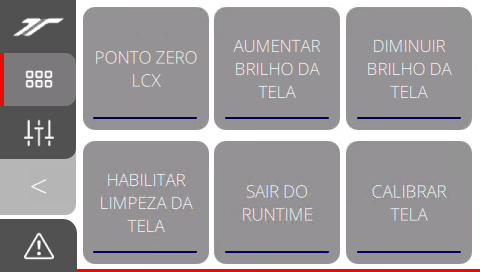
\includegraphics{src/imagesFlexo/11-IHMALM/e-3.png}
\end{figure}
\vspace*{\fill}

\newpage
\thispagestyle{fancy}
\vspace*{40 pt}
\subsection{Tela de ajustes pagina 1}\label{ihmAlimentacaoTelaAjustesPagina1}

Para acessar esta tela basta clicar no ultimo botão do menu esquerdo superior (destacado na imagem abaixo). 
A lógica de ajustes é muito parecida com menu JOG eixos da tela de comandos 
\ifmachineType
contagem, Ver: \ref{telaComandoContagemMenuJOGEixos} - \nameref{telaComandoContagemMenuJOGEixos}.
\else
empilhador, Ver: \ref{sec:telaComandosEmpilhadorMovimentoEixos} - \nameref{sec:telaComandosEmpilhadorMovimentoEixos}.
\fi
A diferença é que nesta tela é possível ajustar a velocidade da máquina por meio
de incrementos fixos de 10 caixas por minuto. Também é possivel ajustar o carro esquadrejador, as guias laterais individualmente e em conjunto.
Ao clicar na sigla o nome completo do ajuste é exibido no centro do menu e no caso de movimentos eles se movimentam na direção apresentada no botão clicado,
em velocidade constante até que o botão seja libreado.

Também é possível habilitar a alimentação de chapas, alterar para o modo de alimentação contínua nesta mesma tela, evitando a necessidade de voltar para a tela de comandos.

\vspace*{\fill}
\begin{figure}[h]
  \centering
  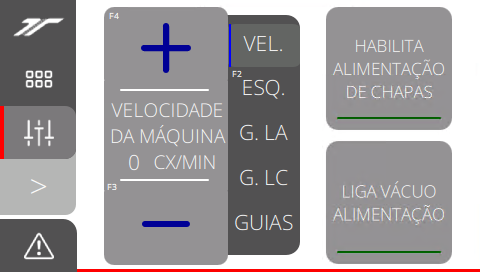
\includegraphics{src/imagesFlexo/11-IHMALM/e-4.png}
\end{figure}
\vspace*{\fill}

\newpage
\thispagestyle{fancy}
\vspace*{40 pt}
\subsection{Tela de ajustes pagina 2}\label{telaAjustes2}
Esta tela é acessada pelo botão "\textgreater" no menu esquerdo superior na tela de comando. A lógica dos outros menus continua sendo a mesma da sua tela "pai" e para voltar a tela anterior basta clicar no botão esquerdo "\textless{}".

Aqui é possível configurar a quantidade de caixas que serão lançadas por vez no modo manual similar a tela de comando alimentação, com diferença que aqui
 para alternar entre os estados de alimentação contínua e alimentação por quantidade de caixas é necessário clicar no botão "Habilita alimentação contínua".
\vspace*{\fill}
\begin{figure}[h]
  \centering
  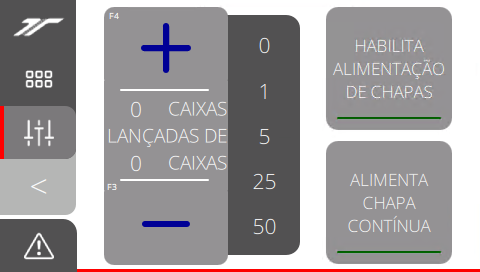
\includegraphics{src/imagesFlexo/11-IHMALM/e-5.png}
\end{figure}
\vspace*{\fill}